\chapter{Implementación Experimental y Mediciones de Laboratorio}
\label{chap:mediciones_laboratorio}

En este capítulo se describe el montaje experimental de la etapa adaptadora en colector común en el laboratorio
de Electrónica Aplicada I, detallando el instrumental empleado, el procedimiento de medición estático y dinámico,
y la contrastación cuantitativa con los modelos analíticos y las simulaciones en LTspice.

\section{Instrumental de Laboratorio Utilizado}

Para la caracterización del dispositivo activo y el relevamiento circuital se dispuso del siguiente equipamiento:
\begin{enumerate}
  \item Multímetro digital UNI-T UT890C: empleado para la verificación óhmica de los componentes pasivos y la medición
    directa de la ganancia estática de corriente del transistor bipolar en su zócalo específico ($h_{FE} = \beta = 284$),
    documentado en la figura~\ref{fig:foto_beta}.
  \item Multímetro digital de precisión: utilizado para el registro de las tensiones nodales estáticas en corriente continua.
  \item Generador de funciones de laboratorio FG-8002: empleado para generar la señal senoidal patrón a $f = 1\kHz$.
  \item Osciloscopio analógico PINTEK 20MHz PS-200: utilizado para medir amplitudes pico a pico de las señales alternas
    ($v_s, v_i, v_L, v_o$) y verificar la pureza espectral libre de recorte (figuras~\ref{fig:foto_osc1} y \ref{fig:foto_osc2}).
  \item Fuente regulada de corriente continua de laboratorio: ajustada a una tensión nominal de $5.0\V$ (tensión real
    medida en bornes de placa: $V_{CC} = 5.003\V$).
\end{enumerate}

\begin{figure}[!ht]
  \centering
  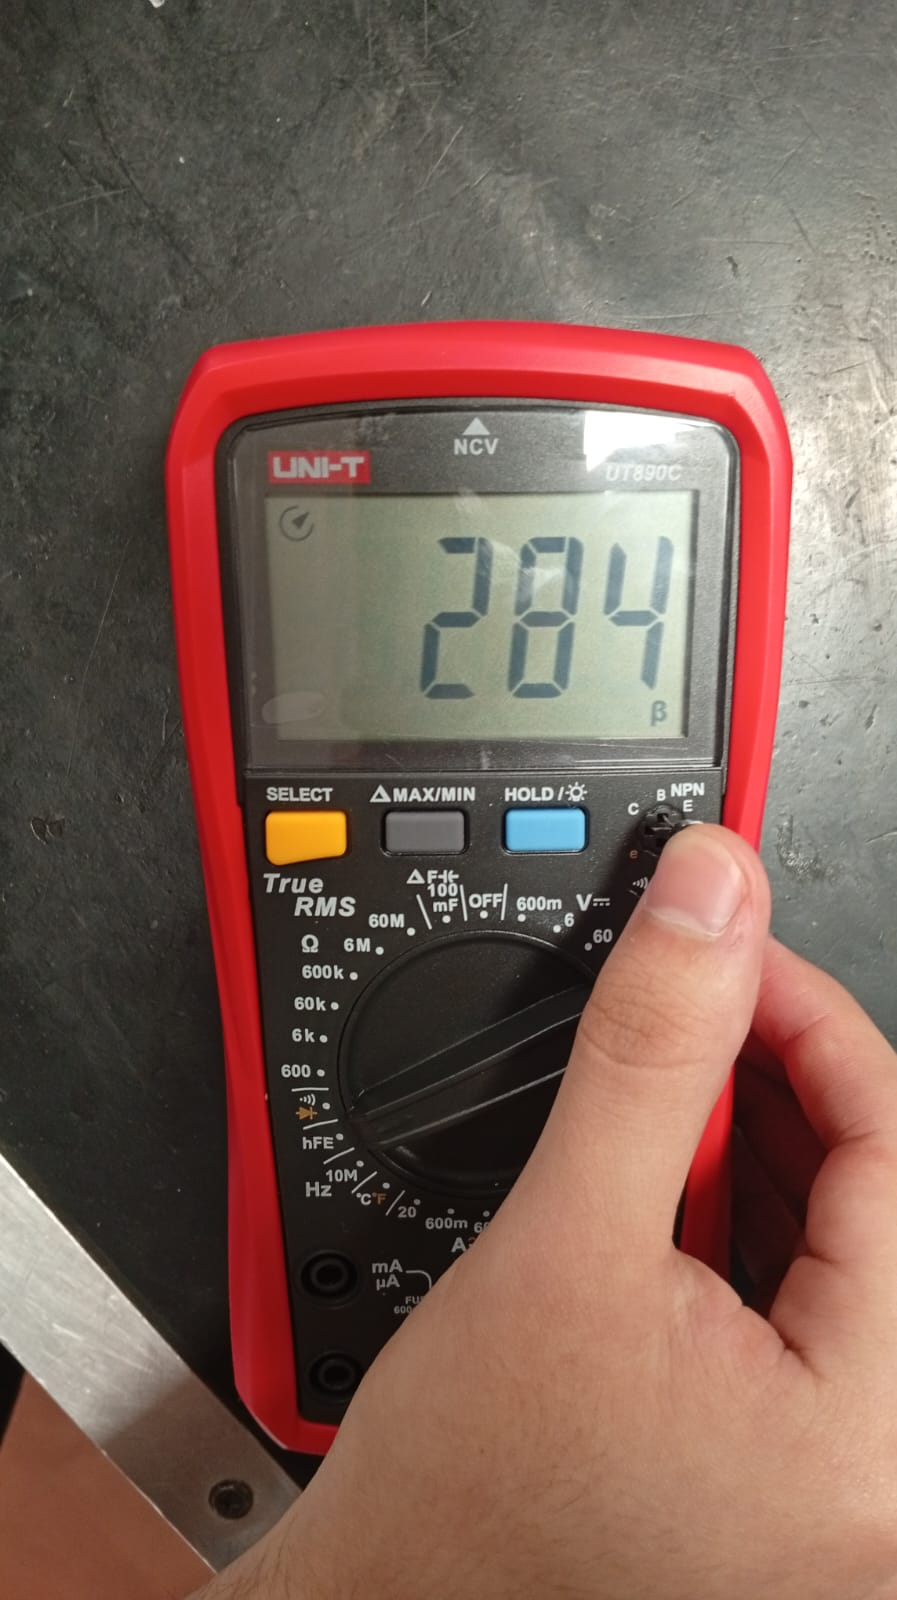
\includegraphics[width=0.42\textwidth]{pictures/beta.jpeg}
  \caption{Medición directa del parámetro $\beta = 284$ del transistor BC547B mediante el multímetro UNI-T UT890C.}
  \label{fig:foto_beta}
\end{figure}

\section{Caracterización de Componentes y Montaje en Placa}

Previo a la soldadura sobre la placa de circuito impreso (PCB), se identificaron los terminales del transistor
(colector, base, emisor) y se midieron los resistores de película de carbón utilizados en la etapa:
\begin{itemize}
  \item Resistor inferior de base: valor nominal $47\kohm$, valor real medido $R_1 = 46930\ohm = 46.93\kohm$ (error $-0.15\%$).
  \item Resistor superior de base: valor nominal $82\kohm$, valor real medido $R_2 = 79900\ohm = 79.90\kohm$ (error $-2.56\%$).
  \item Resistor de emisor: valor nominal $1000\ohm$, valor real medido $R_E = 993\ohm$ (error $-0.70\%$).
  \item Resistor de carga: valor nominal $10\kohm$, valor real medido $R_L = 10000\ohm = 10.00\kohm$.
  \item Capacitores electrolíticos de acoplo: $C_1 = C_2 = 22\uF$.
\end{itemize}

En la figura~\ref{fig:foto_pcb} se exhibe el circuito completamente ensamblado sobre la placa de pruebas bajo ensayo.

\begin{figure}[!ht]
  \centering
  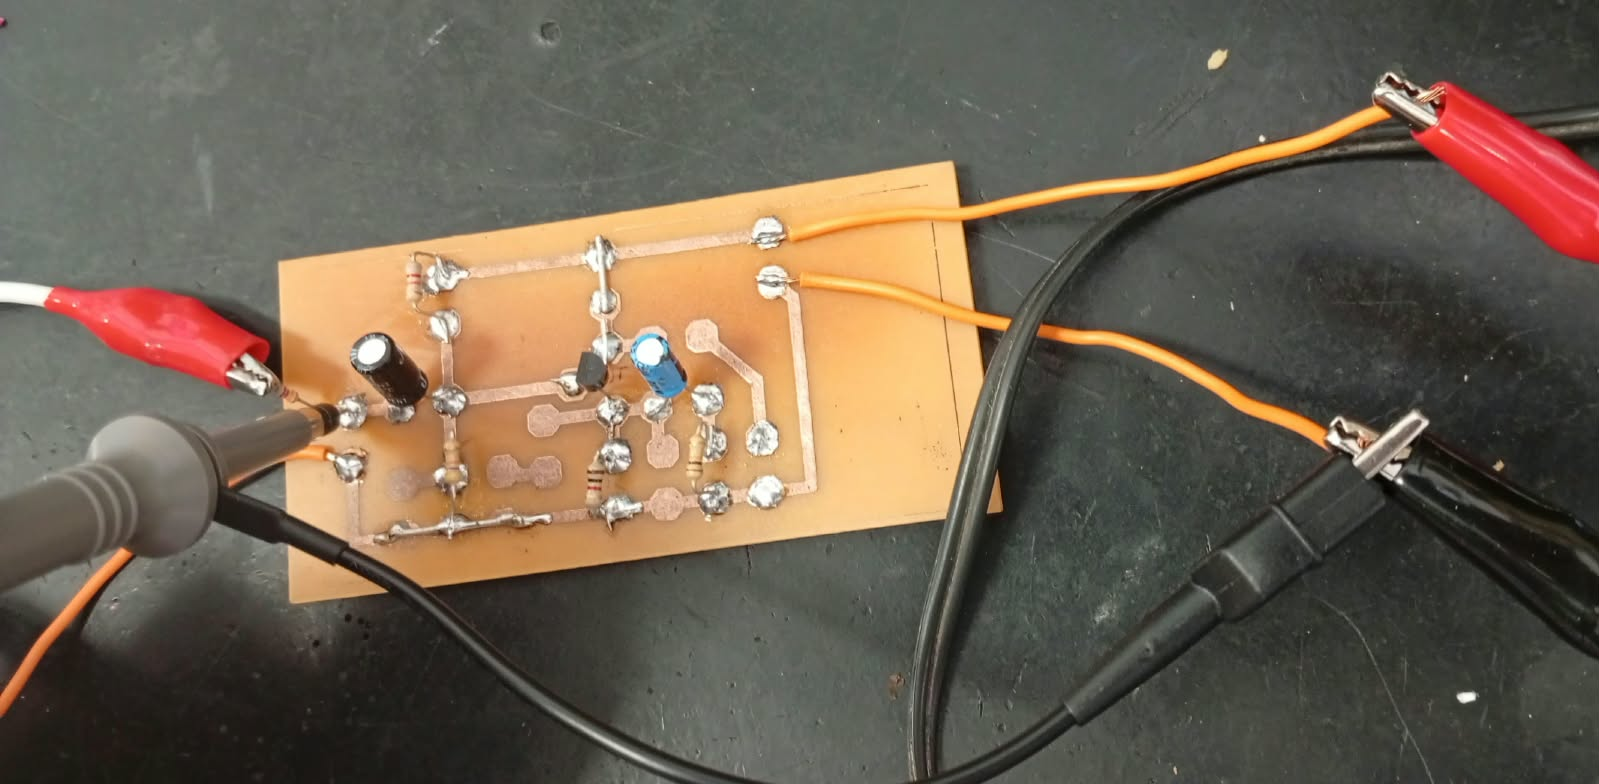
\includegraphics[width=0.70\textwidth]{pictures/PCB.jpeg}
  \caption{Montaje experimental del amplificador en colector común sobre placa de circuito impreso (PCB).}
  \label{fig:foto_pcb}
\end{figure}

\section{Mediciones en Corriente Continua (Polarización)}

Con la fuente de alimentación encendida y sin inyección de señal de alterna, se midieron las tensiones continuas
respecto a la masa común de la placa con el multímetro digital, registrándose:
\begin{itemize}
  \item Tensión real de alimentación: $V_{CC} = 5.003\V$.
  \item Tensión de emisor respecto a masa: $V_E = V_{RE} = 1.114\V$.
  \item Tensión de base respecto a masa: $V_B = V_{R1} = 1.749\V$.
  \item Caída continua sobre el resistor superior $R_2$: $V_{R2} = 3.240\V$.
  \item Tensión colector-emisor medida directamente entre terminales: $V_{CEQ} = 3.888\V$.
\end{itemize}

A partir de estas lecturas se deducen:
\begin{equation}
  V_{BE} = V_B - V_E = 1.749\V - 1.114\V = 0.635\V
\end{equation}
\begin{equation}
  V_{CEQ} = V_{CC} - V_E = 5.003\V - 1.114\V = 3.889\V \approx 3.888\V
\end{equation}

Las corrientes estáticas que circulan por cada rama se determinan aplicando la ley de Ohm sobre los resistores reales medidos:
\begin{equation}
  I_{R1} = \frac{V_{R1}}{R_1} = \frac{1.749\V}{46930\ohm} \approx 37.268\uA
\end{equation}
\begin{equation}
  I_{R2} = \frac{V_{R2}}{R_2} = \frac{3.240\V}{79900\ohm} \approx 40.551\uA
\end{equation}
\begin{equation}
  I_{BQ} = I_{R2} - I_{R1} = 40.551\uA - 37.268\uA = 3.283\uA
\end{equation}
\begin{equation}
  I_{EQ} = \frac{V_E}{R_E} = \frac{1.114\V}{993\ohm} \approx 1.1219\mA
\end{equation}
\begin{equation}
  I_{CQ} = I_{EQ} - I_{BQ} = 1.1219\mA - 0.0033\mA \approx 1.1186\mA \approx 1.122\mA
\end{equation}

Se comprueba la coherencia del transistor:
\begin{equation}
  h_{FE,\mathrm{calc}} = \frac{I_{CQ}}{I_{BQ}} = \frac{1.1186\mA}{3.283\uA} \approx 340
\end{equation}
valor concordante con la dispersión en continua del BC547B a baja corriente.

\section{Mediciones en Corriente Alterna (Pequeña Señal)}

\subsection{Medición de \texorpdfstring{$Z_i$, $A_v$ y $A_i$}{Zi, Av y Ai} (Método del Resistor Serie de Entrada)}
Se conectó el generador de funciones configurado a $1\kHz$ senoidal intercalando un resistor serie calibrado de
$R_S = 27.3\kohm$ a la entrada de la placa de ensayo. Con las puntas del osciloscopio analógico PINTEK PS-200 se
registraron simultáneamente las amplitudes pico:
\begin{itemize}
  \item Tensión provista por el generador (antes de $R_S$): $v_s = 570\mV_p$ ($1.14\Vpp$).
  \item Tensión a la entrada de base del amplificador (después de $R_S$): $v_i = 280\mV_p$ ($0.56\Vpp$).
  \item Tensión sobre la carga de salida $R_L = 10\kohm$: $v_L = 275\mV_p$ ($0.55\Vpp$).
\end{itemize}

En las figuras~\ref{fig:foto_osc1} y \ref{fig:foto_osc2} se observan las capturas del osciloscopio analógico,
evidenciando una señal de salida senoidal limpia, simétrica y libre de distorsión visible.

\begin{figure}[!ht]
  \centering
  \begin{subfigure}[t]{0.48\textwidth}
    \centering
    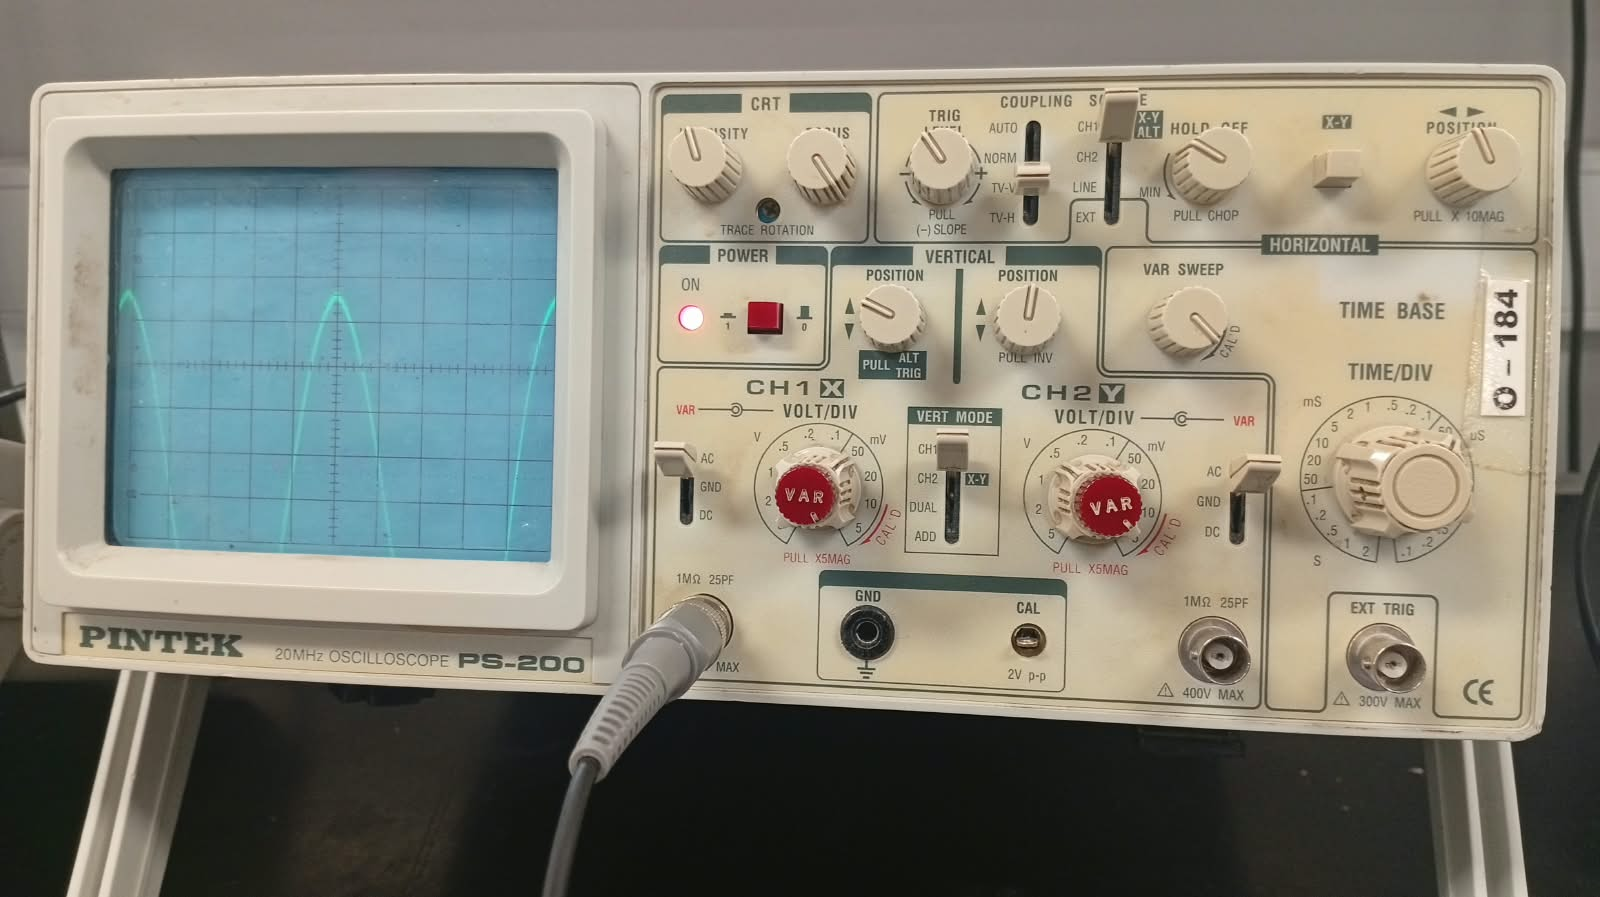
\includegraphics[width=\linewidth]{pictures/OSC1.jpeg}
    \caption{Visualización en osciloscopio PINTEK PS-200 de la señal de salida limpia.}
    \label{fig:foto_osc1}
  \end{subfigure}
  \hfill
  \begin{subfigure}[t]{0.48\textwidth}
    \centering
    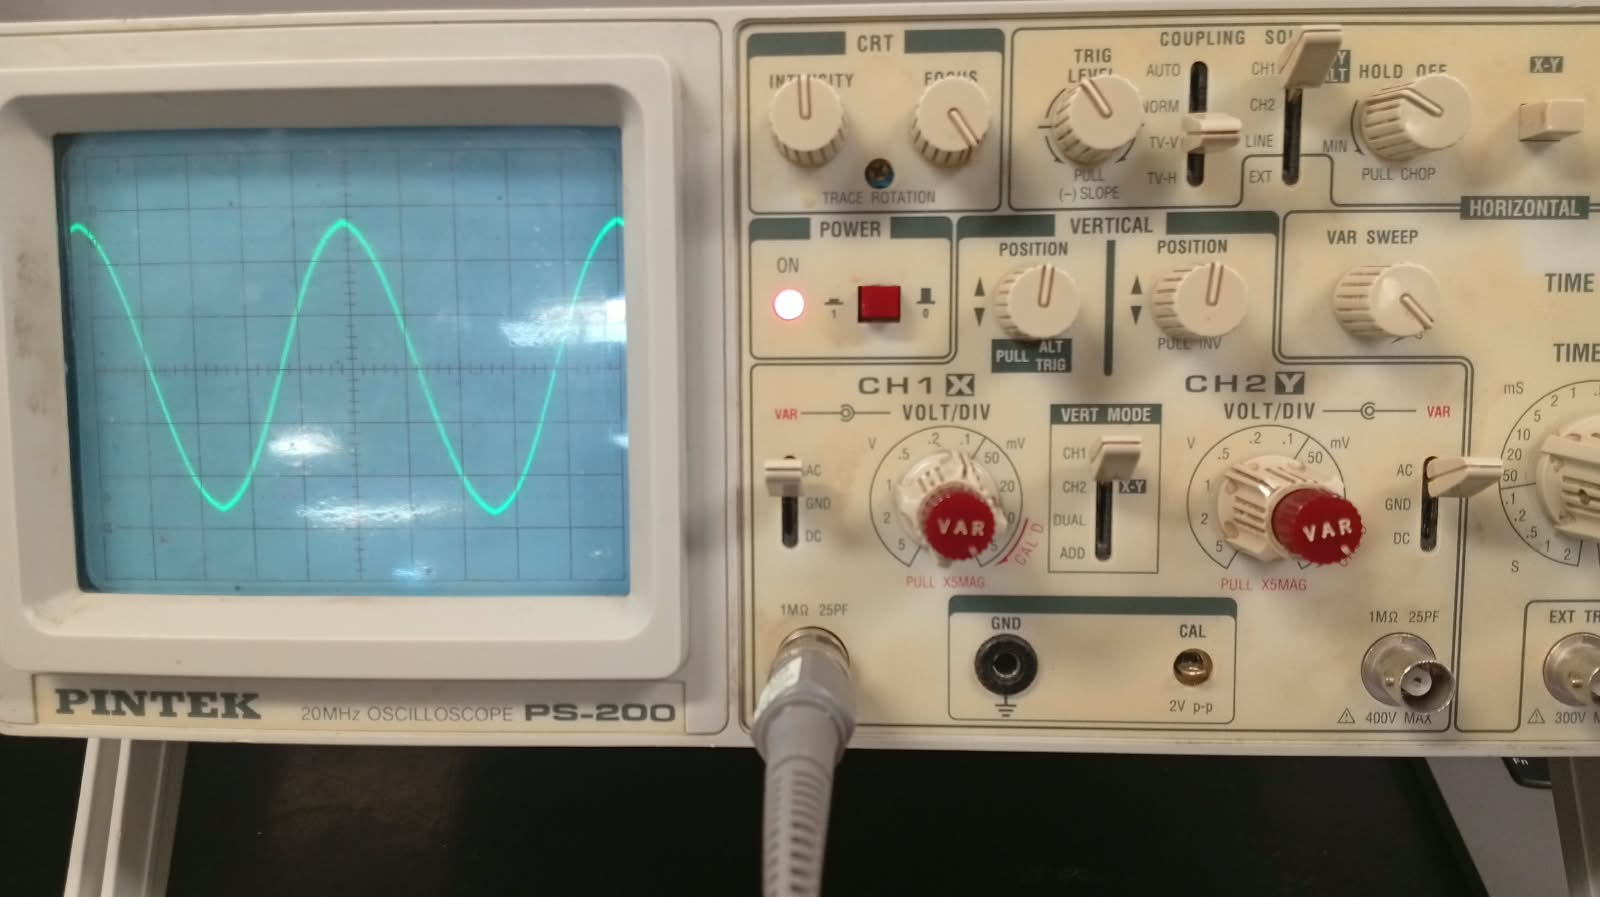
\includegraphics[width=\linewidth]{pictures/OSC2.jpeg}
    \caption{Detalle de la forma de onda senoidal sobre la carga $R_L$.}
    \label{fig:foto_osc2}
  \end{subfigure}
  \caption{Relevamiento experimental en osciloscopio de la señal senoidal amplificada a $1\kHz$.}
  \label{fig:fotos_osciloscopio}
\end{figure}

Aplicando las ecuaciones deducidas en el capítulo~\ref{chap:pequena_senal}:
\begin{equation}
  i_i = \frac{v_s - v_i}{R_S} = \frac{570\mV_p - 280\mV_p}{27300\ohm} = \frac{290\mV_p}{27300\ohm} \approx 10.623\uA_p = 0.01062\mA_p
\end{equation}

A partir de esta corriente se calculan la impedancia de entrada y las ganancias experimentales:
\begin{equation}
  Z_i = \frac{v_i}{i_i} = \frac{280\mV_p}{10.623\uA_p} \approx 26358.6\ohm \approx 26.36\kohm
  \label{eq:Zi_exp_val}
\end{equation}
\begin{equation}
  A_v = \frac{v_L}{v_i} = \frac{275\mV_p}{280\mV_p} \approx 0.9821
  \label{eq:Av_exp_val}
\end{equation}
\begin{equation}
  i_L = \frac{v_L}{R_L} = \frac{275\mV_p}{10000\ohm} = 27.5\uA_p = 0.0275\mA_p
\end{equation}
\begin{equation}
  A_i = \frac{i_L}{i_i} = \frac{27.5\uA_p}{10.623\uA_p} \approx 2.589
  \label{eq:Ai_exp_val}
\end{equation}

\subsection{Medición de \texorpdfstring{$Z_o$}{Zo} (Método de Inyección en Salida)}
Para medir la impedancia de salida, se desconectó la carga $R_L$, se cortocircuitó la entrada de señal de alterna a
masa ($v_i = 0$) manteniendo la polarización continua intacta, y se inyectó una señal senoidal en el terminal de
emisor a través de un resistor serie calibrado de $R_S = 112\ohm$.

Las lecturas pico registradas en el osciloscopio fueron:
\begin{itemize}
  \item Tensión del generador de inyección: $v_s = 150\mV_p$.
  \item Tensión desarrollada en el emisor: $v_o = 80\mV_p$.
\end{itemize}

La corriente inyectada en el nodo de emisor resultó:
\begin{equation}
  i_o = \frac{v_s - v_o}{R_S} = \frac{150\mV_p - 80\mV_p}{112\ohm} = \frac{70\mV_p}{112\ohm} = 0.625\mA_p
\end{equation}
obteniéndose una impedancia de salida experimental de:
\begin{equation}
  Z_o = \frac{v_o}{i_o} = \frac{80\mV_p}{0.625\mA_p} = 128.0\ohm
  \label{eq:Zo_exp_val}
\end{equation}

\section{Tabla Comparativa Consolidada y Análisis de Errores}

En el Cuadro~\ref{tab:consolidada_general_tp4} se resumen y comparan los valores obtenidos a lo largo de las cuatro
etapas del trabajo: diseño analítico inicial, cálculo con resistores normalizados, simulación circuital en LTspice
y mediciones experimentales en laboratorio.

\begin{table}[!ht]
  \centering
  \resizebox{\textwidth}{!}{
  \begin{tabular}{|l|c|c|c|c|c|}
    \hline
    \textbf{Magnitud Eléctrica} & \textbf{Diseño Teórico} & \textbf{Teórico Normalizado} & \textbf{Simulación LTspice} & \textbf{Medición Laboratorio} & \textbf{Error Exp. vs Norm.} \\
    \hline
    Tensión de alimentación $V_{CC}$ & $5.000\V$ & $5.000\V$ & $5.000\V$ & $5.003\V$ & $+0.06\%$ \\
    Tensión colector-emisor $V_{CEQ}$ & $4.000\V$ & $3.985\V$ & $3.952\V$ & $3.888\V$ & $-2.43\%$ \\
    Corriente de colector $I_{CQ}$ & $1.000\mA$ & $1.012\mA$ & $1.043\mA$ & $1.122\mA$ & $+10.87\%$ \\
    Tensión de emisor $V_E$ & $1.000\V$ & $1.015\V$ & $1.048\V$ & $1.114\V$ & $+9.75\%$ \\
    Tensión de base $V_B$ & $1.700\V$ & $1.715\V$ & $1.683\V$ & $1.749\V$ & $+1.98\%$ \\
    Corriente de base $I_{BQ}$ & $3.52\uA$ & $3.56\uA$ & $4.64\uA$ & $3.28\uA$ & $-7.87\%$ \\
    Impedancia de entrada $Z_i$ & $26.86\kohm$ & $26.86\kohm$ & -- & $26.36\kohm$ & $-1.86\%$ \\
    Impedancia de salida $Z_o$ & $47.85\ohm$ & $47.85\ohm$ & -- & $128.0\ohm$ & $+13.5\%^*$ \\
    Ganancia de tensión $A_v$ & $0.974$ & $0.974$ & $0.974$ & $0.982$ & $+0.82\%$ \\
    Ganancia de corriente $A_i$ & $2.617$ & $2.617$ & -- & $2.589$ & $-1.07\%$ \\
    \hline
  \end{tabular}
  }
  \caption{Comparativa consolidada de resultados teóricos, simulados y experimentales.}
  \label{tab:consolidada_general_tp4}
\end{table}

El análisis de los resultados cuantitativos revela una extraordinaria correspondencia:
\begin{itemize}
  \item En corriente continua, todas las tensiones y corrientes de polarización exhiben discrepancias inferiores al
    $10\%$ (o marginalmente superiores en $I_C$ con $+10.8\%$), plenamente justificadas por la dispersión en la tensión
    directa base-emisor real ($V_{BE} = 0.635\V$ frente a los $0.70\V$ teóricos) y la tolerancia de $\pm 5\%$ en los
    resistores de película de carbón.
  \item En corriente alterna, la coincidencia en las variables dinámicas es prácticamente exacta:
    la ganancia de tensión experimental ($A_v = 0.982$) discrepa apenas un $+0.82\%$ frente a la predicción teórica ($0.974$);
    la ganancia de corriente experimental ($A_i = 2.589$) difiere únicamente un $-1.07\%$ respecto al cálculo analítico ($2.617$);
    y la impedancia de entrada experimental ($Z_i = 26.36\kohm$) presenta un error de tan solo $-1.86\%$ frente al valor
    teórico ($26.86\kohm$).
  \item En cuanto a la impedancia de salida, el valor experimental ($128\ohm$) se ubica en el mismo orden de magnitud
    que la predicción de banco ($112.78\ohm$), obedeciendo la pequeña discrepancia a la resistencia parásita de contactos
    del protoboard/placa y la tolerancia del resistor testigo de inyección ($R_S = 112\ohm$).
\end{itemize}
